\chapter{Random variables}
\begin{definition}
    In a Borel space \borel, a random variable is a function $X:\Omega \to \bbR$ s.t. for all $x \in \bbR$ the set $\{\omega \in \Omega : X(\omega) \le x\} \in \eff$.
\end{definition}

\begin{example}
    I toss a coin five times. This is a random experiment and the sample space can be written as
    \begin{equation*}
        S=\{TTTTT,TTTTH,\ldots,HHHHH\}.
    \end{equation*}
    Note that here the sample space S has $2^5=32$ elements. Suppose that in this experiment, we are interested in the number of heads. We can define a random variable X whose value is the number of observed heads. The value of X will be one of 0,1,2,3,4 or 5 depending on the outcome of the random experiment.
\end{example}
\begin{example}
    Fix $c \in \bbR\text{. } X(\omega) \equiv c \; \forall \omega \in \bbR$. $X$ is a \textbf{degenerate random variable}.
    \begin{equation*}
        \text{Pick } a \in \bbR\text{. }
        P(X=a)=\begin{cases*}
            1 & a = c\\
            0 & a \ne{} c
        \end{cases*}
    \end{equation*}
\end{example}
Not only we can check that the probability that a random variable is equal to a fixed value, but we can also check the probability that the random variable gives as results values in an interval.\\
Let's consider \probspace{} a probability space, $X:\Omega\to\bbR$ a random variable, and $A \in \calB$ ($\calB$ is a Borel \sigal{}, that is the smallest family of subsets in $\bbR$ that contains all the intervals and checks the properties of being a \sigal). Then
\begin{equation*}
    P(X \in A) = P(\{\omega \in \Omega:X(\omega)\in A\})
\end{equation*}
The function $X:\borel\to (\bbR, \calB)$ transforms the probabilities $P$ defined on the Borel space \borel{} to values in $(\bbR, \calB)$. We can denote this probability measure with $P_X$.
\begin{definition}
    Given a probability space \probspace{} and a random variable $X:\borel\to (\bbR, \calB)$, the law or \textbf{distribution} of $X$ is the probability function $P_X$ defined on $(\bbR, \calB)$ for all $A \in \calB$ as
    \begin{equation*}
        P_X(A) \coloneq P(X \in A) = P(\{\omega \in \Omega:X(\omega)\in A\})=P(X^{-1}(A))
    \end{equation*}.
\end{definition}
\begin{example}
    Let \probspace{} be a probability space, $E \in \eff$. Let's consider an urn with 50 white marbles and 50 black ones. The \textbf{indicator random variable} X tells us if $\omega$ is in the set of the event $E$ (ex. "i pick a black marble") by returning a zero or a one. Let $E$ be the event "the marble drawn is white".
    \begin{equation*}
        X = I_E(\omega)=\mathbb{1}_E(\omega)=\begin{cases*}
            1 & if $\omega \in E$\\
            0 & if $\omega \in E^C$
        \end{cases*}
    \end{equation*}
    Then for $A \in \calB$,
    \begin{equation*}
        P_X(A)=P(X \in A) = \begin{cases*}
            1 & if if $0 \in A$ and $1 \in A$\\
            \frac{1}{2} & if $0 \in A$ and $1 \notin A$\\
            \frac{1}{2} & if $0 \notin A$ and $1 \in A$\\
            0 & if $0 \notin A$ and $1 \notin A$
        \end{cases*}
    \end{equation*}
\end{example}
This tells us the following: if I choose the event $E=\text{"I pick a black marble"}$ as the indicator and a set $A$ with real numbers inside, then:
\begin{itemize}
    \item There is probability $1$ that the event happens ($1 \in A$) or doesn't happen ($0 \in A$)
    \item There is probability $\frac{1}{2}$ that the event happens ($0 \notin A \text{ and } 1 \in A$)
    \item There is probability $\frac{1}{2}$ that the event doesn't happen ($0 \in A \text{ and } 1 \notin A$)
    \item There is probability $0$ that the the random variable gives as result a number different from 0 and 1 ($0 \notin A \text{ and } 0 \notin A$)
\end{itemize}
Now we may be interested at what happens if we progressively sum the probabilities by taking a set that starts from $-\infty$ and making its right boundary vary.
\begin{definition}
    Given a random variable $X$, the \textbf{cumulative distribution function (cdf)} of $X$ is the function $F_X:\bbR\to\bbR$ defined for all $t \in \bbR$ s.t.
    \begin{equation*}
        \begin{split}
            F_X(t) & = P(X\le t)\\
            & = P_X((-\infty, t])\\
            & = P(X \in (-\infty, t])\\
            & = P(\{\omega\in\Omega:X(\omega)\le t\})
        \end{split}
    \end{equation*}
\end{definition}
\begin{figure}[ht]
    \centering
    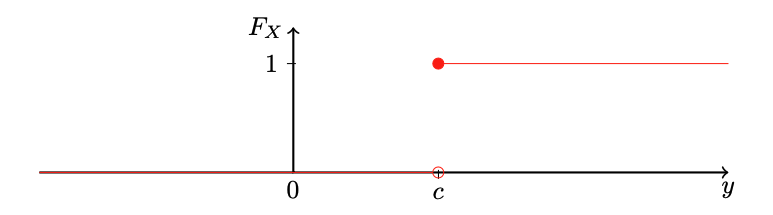
\includegraphics[width=0.6\textwidth]{images/cumulative.png}
    \caption*{Cumulative distribution function of the degenerate random variable $X\equiv c$}
\end{figure}
\begin{figure}[ht]
    \centering
    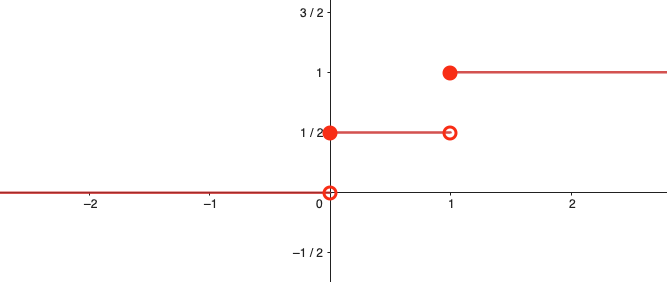
\includegraphics[width=0.61\textwidth]{images/cumulative1.png}
    \caption*{Cumulative distribution function from the marbles exercise}
\end{figure}
\vbox{
    Properties of $F_X$:
    \begin{enumerate}
        \item $F_X(\bbR) = [0, 1]$
        \item $\lim_{x \to -\infty} F_X=0, \lim_{x \to +\infty} F_X=1$
        \item non-decreasing
        \item cadlag: continuous to the right ($\lim_{x \to x_0^+} f(x) = f(x_0)$), limited to the left ($\lim_{x \to x_0^-} $ exists on $[0, 1]$)
    \end{enumerate}
}
As it can be seen from the graphs, the height of the jump at point $x_0$ represents the probability of the set of elements of $\Omega$ that have the random variable equal to $x_0$.
\section{Discrete random variables}
\begin{definition}
    A discrete random variable is a random variable returning a finite or countable number of values.
\end{definition}
\begin{remark}
    A random variable is discrete iff its distribution function is discontinuous and piecewise constant, with at most a countable number of discontinuities. These discontinuity points are the values that the random variable can take.
\end{remark}
\begin{definition}
    Let $X$ be a discrete r. v. We define the function $\rho_X:\bbR\to[0,1]$ called \textbf{probability mass function (pmf)} or absolute density of $X$ as
    \begin{equation*}
        \rho_X(k)=P(X=k)=P(\{\omega \in \Omega:X(\omega)=k\}) \; k\in\bbR.
    \end{equation*}
\end{definition}
\begin{definition}
    $\calR_X$ is the set of all the images of $X$.
    \begin{equation*}
        \calR_X=\{x \in \bbR: \rho_X(x)\ne 0\}
    \end{equation*}
\end{definition}
Properties of $\rho_X$:
\begin{enumerate}
    \item $\rho_X \in [0, 1]$
    \item $\forall x \in \calR_X^c, \rho_X(x)=0$
    \item $\sum_{x \in \calR_X}\rho_X(x)=1 $
    \item if $E \in \calB$, then $P_X(E)=\sum_{x \in \calR_X\cap E}\rho_X(x)=\sum_{x \in \calR_X}\mathbb{1}_E(x)\rho_X(x)$
    \item $F_X(t)=P_X((-\infty,t])=\sum_{x \in \calR_X}\mathbb{1}_{(-\infty, t)}(x)\rho_X(x)$
\end{enumerate}
\begin{figure}[ht]
    \centering
    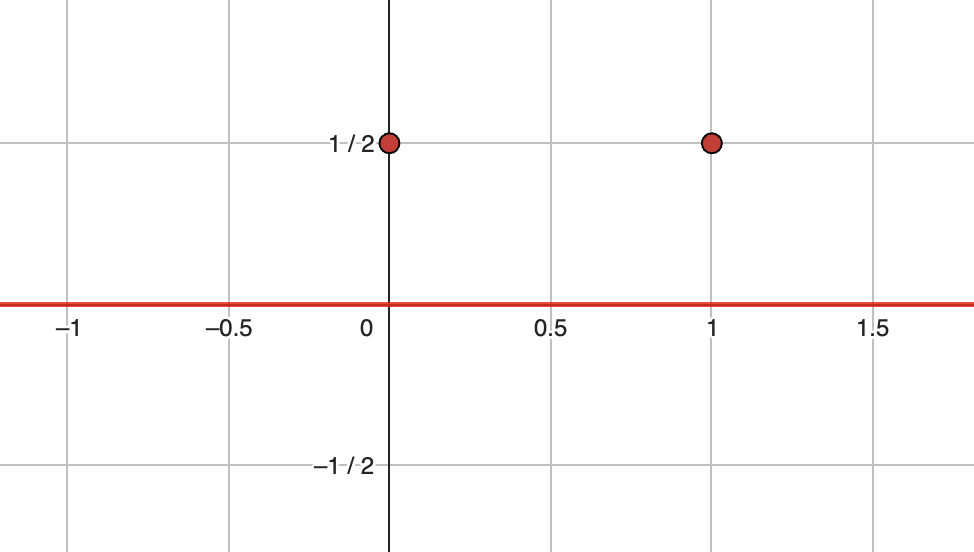
\includegraphics[width=0.6\textwidth]{images/pmf.png}
    \caption*{pmf of the marbles exercise}
\end{figure}
\section{Absolutely continuous random variables}
\begin{definition}
    A random variable $X$ is continuous if the distribution function $F_X$ is continuous. If additionally there exists a non-negative function $f_X:\bbR\to\bbR$ s.t. $\forall x\in\bbR$,
    \begin{equation*}
        F_X(x)=\int_{-\infty}^{x} f_X(y) \,dy
    \end{equation*}
    then $X$ is absolutely continuous.
\end{definition}
We can't define a probability mass function for continuous functions, because since $F_X$ is continuous (it has no jumps), for all $x \in \bbR$ we have $P(X=x)=0$ and $\rho_X$ would be 0. Instead, we can usually define the probability density function (pdf). The pdf is the density of probability rather than the probability mass. The concept is very similar to mass density in physics: its unit is probability per unit length.
\begin{definition}
    Let $X$ be an absolutely continuous random variable. By definition, there exists a non- negative function $F_X(x)=\int_{-\infty}^{x} f_X(y) \,dy$. This function $f_X$ is the probability density function (pdf), sometimes shortened to density, of $X$.
\end{definition}
\begin{remark}
    In the points where $F_X$ is differentiable, $F_X'=f(x)$.
\end{remark}
\begin{remark}
    $F_X$ can be $>1$, since it is not a probability.
\end{remark}